
Recent GDELT updates provide feeds with 15-minute resolution \cite{GDELT2}, but historical feeds offered only daily resolution. We decided for simplicity to analyze daily changes in price, taking a full day's worth of news data into account. This was most in line with testing our hypothesis, that an aggregation of topic clusters in a day's news is predictive of commodity pricing.

Our data pipeline was designed to provide day-wise parallelism over our data set in order to enable fast testing of new feature extraction methods. The raw data, as well as intermediate data, is stored in TSV ASCII format.

\subsection{Model}

Every news event in GDELT is stored as a row in a file for that day's report. Every set of rows may undergo a series of transformations. First, in the \textbf{preprocessing} stage, we extract relevant topic- and importance- related columns. For topics, a mix of numeric and categorical fields are extracted. Importance columns are saved for use in a further step. Next, in the \textbf{expansion} stage, we project each row of topic features to a purely real space by using one-hot encoding for categorical values. For each category, one-hot encoding assigns an integer to each unique value in that category. Finally, in the \textbf{summary} stage, $K$-means clustering is performed on this purely numeric representation of the data. Euclidean distance is used as the distance metric for $K$-means. A range of values between 10 and 5000 are used for $K$.

The day summaries are then conglomerated in a time series $\{\textbf{d}_i\}$. For a day-indexed time series of a commodity's price, $\{p_i\}$, we have the corresponding sequence of binary labels indicating whether price has increased the next day, $y_i=1_{p_{i+1}>p_i}$.

Thus, our model assumes that:
\begin{enumerate}
\item The static clustering of news topics is accurate for the future.
\item $\mathbb{P}(p_{i+1}>p_i)$ may be determined by a regression over summaries $\textbf{d}_i$. 
\end{enumerate}

Both of these are strong assumptions. The first may be weakened by adapting a dynamic clustering model, such as an infinite Gaussian Mixture Model or an HDP. The second requires $\textbf{d}_i$ to be both contain a sufficient amount of information to predict price behavior, which is a matter of appropriate feature extraction, and the assumption that we do not lose too much predictive power in summarizing a day by aggregating over the clusters to which its news events belonged to.

\subsubsection{Autoregressive Models: ARMA}
AR models are some of the most flexible and easy to use models for time series. They have proven to be especially useful for describing the dynamic behavior of economic and financial time series and for forecasting \cite{tsay, VAR} TODO(Sean): fix citation. \\
The basic p-lag vector autoregressive model (AR(p)) has the form: $$\bf{Y}_t=\bf{c}+\bf{\Pi}_1\bf{Y}_{t-1}+\bf{\Pi}_2\bf{Y}_{t-2}+\cdots+\bf{\Pi}_p\bf{Y}_{t-p}+\epsilon_t,$$ $$t=1\ldots T$$ with $\Pi_i$ being the coefficients and $\epsilon_t$ is an unobservable zero mean noise. We can also do subset-autoregression where we pick specific lags.
One of the most common extensions to Autoregressive models is to include moving averages and integration terms that take into account the stationarity of the time series. This is what constitutes Auto-Regressive Integrated Moving Average (ARIMA) models. They are  the most general class of models for forecasting a time series which can be made to be “stationary” by differencing (if necessary), perhaps in conjunction with nonlinear transformations. 
Determining the order of the lags and moving average can be done either graphically using an Autocorrelation Function plot (in addition to a Partial Autocorrelation Function plot) [Figure \ref{fig:ACF}] or analytically using a goodness of fit measure. ACF or PACF plots indicates which lags are most correlated within the time series. Additionally, there are a few tricks that we didn't use to determine MA terms from the PACF plot.
\begin{figure}[ht]
	\vskip 0.2in
	\begin{center}
		\centerline{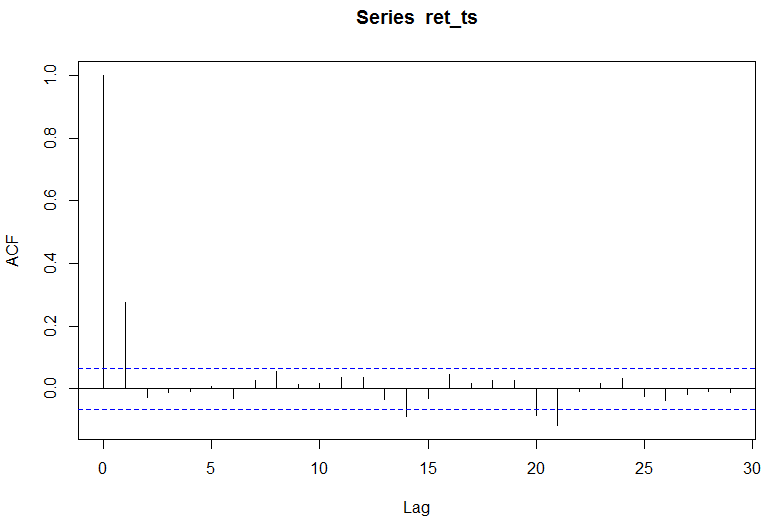
\includegraphics[width=\columnwidth]{ACF.png}}
		\caption{Autocorrelation Function plot for gold. Lags exceeding the dotted blue line have a significant autocorrelation. As we can see, the lag at 1, 14, 20 and 21 are autocorrelated.}
	\end{center}
	\vskip -0.2in
	\label{fig:ACF}
\end{figure}
For the goodness of fit, we decided to use the Akaike information criterion (AIC) which evaluates models, relative to each other. AIC aims to choose a model which minimizes the KL divergence between the true density and the density of the MLE such that the best model is the one with the lowest AIC. However, AIC is prone to overfitting and chooses predictive models over parsimonious ones.
For the order of integration, note that a random variable that is a time series is stationary if its statistical properties are all constant over time.  A stationary series has no trend, its variations around its mean have a constant amplitude, and it wiggles in a consistent fashion, i.e., its short-term random time patterns always look the same in a statistical sense. \cite{tsay, VAR}
One can verify the non-stationarity hypothesis using an Augmented Dickey Fuller (ADF). In our case, we had a p-value of 0.01 which rejects non-stationarity and confirms that there is no trend in our time series data.
Additionally, it is easy to simulate the AR coefficients of ARIMA using simple linear models that include the lags as independent variables. This can be less powerful
Note that we didn't use Markov Switching which is a model that assumes the existence of latent regimes and builds an independent model for each regime because.\cite{MS} After testing, we couldn't find any significant regimes in our training data which might infer that our regimes are over longer periods of time than that spanned by our data.
\subsubsection{News Data: Exogenous Factors}
There have been 2 standard methods to include exogenous factors (factors from outside the system of the time series): analyzing the impluse responses in the time series with respect to events that occured at the same time or simply including them as an extra independent regressor in the model. Given the complexity of impulse responses we decided to use an ARIMAX model (ARIMA + Exogenous factors) that includes our news data columns as regressors that we can select from based on their statistical significance as well as their correlation.
However, with around 800 columns for the model with 100 clusters, we can easily overfit random data points to our noisy news columns which can throw us off in the training and cause disastrours out-of-sample results.
\subsubsection{Column Selection of News Data}
ARIMA and OLS regression require the number of features to be less than or equal to the number of observations which can be problematic when we try to test smaller training window sizes. Therefore, we recurred to Principal Component Analysis (among other methods that we tried). PCA converts a set of observations of possibly correlated variables into a set of values of linearly uncorrelated variables called principal components.\cite{PCA} In our case, we extracted the principal components that account for $99\%$ of the variance in our data and used those for the training.
\subsubsection{L1-regularization: Lasso Regression}
In order to avoid overfitting the data as well as to enable the usage of window sizes that are smaller than the number of explanatory variables (because, otherwise the design matrix for OLS), we resorted to Lasso regression.\cite{glmnet} It allows the reduction of columns while considering their correlation to the response variable, unlike PCA. Lasso regression yields a sparse solution (many of the coefficients are zeros) which helps to avoid overfitting, that we noticed clearly in ARIMA and simple linear models. Additionally, Lasso is computationally efficient as compared to other sparse regressions.\cite{glmnet} Finally, we can select the degree of our sparsity by selecting a Lambda coefficient which helps us better gauge the change of the predictive power of our model.
Accordingly, we build Lasso model with the minimum Lambda as defined by cross-validation and then use that model to estimate our log-returns for each training window.
\subsubsection{Testing Measures}
For out-of-sample testing, we used two measures. The first is Mean Absolute Error which describes the difference in absolute value between our predictions and actual values. The closer MAE is to 0, the better we fit the data quantitatively. However, for our final purpose of designing a trading strategy, it could be good enough to detect if the stock is going up or down. In this case, predicting the binary values is what we seek. Accordingly, we would convert our predictions to binary based on their sign (positive log returns implies an increase from last day) and use simple binary-classification measures such as accuracy and F-1. We focused on the accuracy rate because we have almost equal amount of positive and negative data points that we are not biased by the training which is usually the point at which one needs to use F1-score.
\subsubsection{Training the Time Series}
We split our data into adjacent (to preserve the temporal order) training and testing windows of varying sizes as can be seen in the results section. We also resorted to moving window training (also called walk-forward optimization) which is a form of k-fold cross-validation for time series data. We have a moving window of the time series and at each instance of the window we re-estimate the coefficients (not the order but the coefficients given the fixed order). This is contrast to a fixed-window for training such that you use the same coefficients for every prediction. Accordingly, moving-window training would have a higher predictive power since the model changes as the window moves and thus carries more weight as the predictions go further in time. With a fixed window, the further the predictions are, the less relevant is the model from the fixed window since it's based on data that is too old.
This was one of the trade-offs we had to decide on. The second was figuring out the best ARIMA order (MA, I and AR orders) which takes a few hours at a time: do we re-estimate for each window or build it on a single window and assume orders don't change too much? therefore, it would take a long time to re-estimate the order for every training window.
Accordingly, we ended up doing a moving-window training strategy that looks ahead one step at a time and re-estimates the coefficients at each time but uses the same orders (number of lags and ma coefficients).	

\subsection{Execution}

Our current implementation uses $K$-means for clustering and logistic regression for classification. We trained, validated, and sampled from the days between 2006-01-01 and 2015-07-31. Recent days were used for testing.

For our random sample, we sampled one million total events, with rate from a day's file proportional to the number of events in that day. The random sample undergoes the same preprocessing and expansion pipeline as described below for the day summaries to be used in the regression, but its output is fed into a clustering model, that is then used in the main pipeline. We are forced to use a sample for tractability.

Raw data starts with 58 columns. Each day typically has 100K rows. The total size of the set is about 60GB. %TODO precise mean and stddev.

\begin{figure}[ht]
\vskip 0.2in
\begin{center}
\centerline{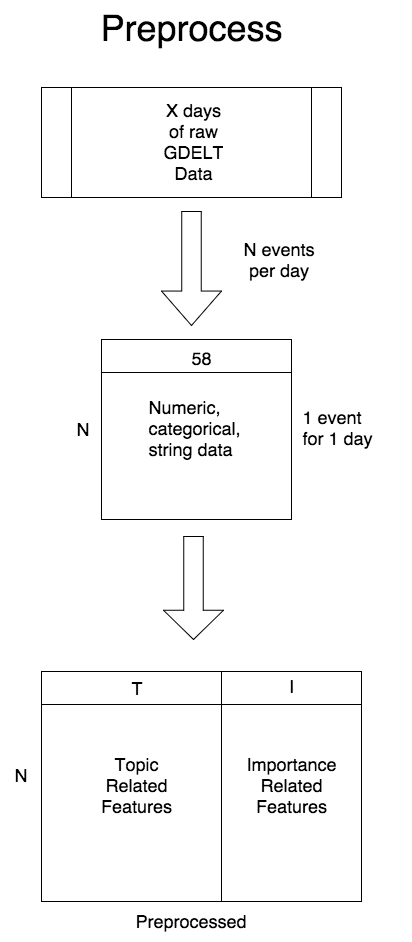
\includegraphics[scale=0.15]{images/preprocess_vertical.png}}
\caption{Preprocessing stage}
\end{center}
\vskip -0.2in
\label{fig:preprocess}
\end{figure}

After preprocessing, we are left with $T=12$ topic-related columns and $I=9$ importance columns, where the topic columns are in a compressed format, with categorical variables represented as integers and strings still as strings (though now sanitized and with stop words removed).

\begin{figure}[ht]
\vskip 0.2in
\begin{center}
\centerline{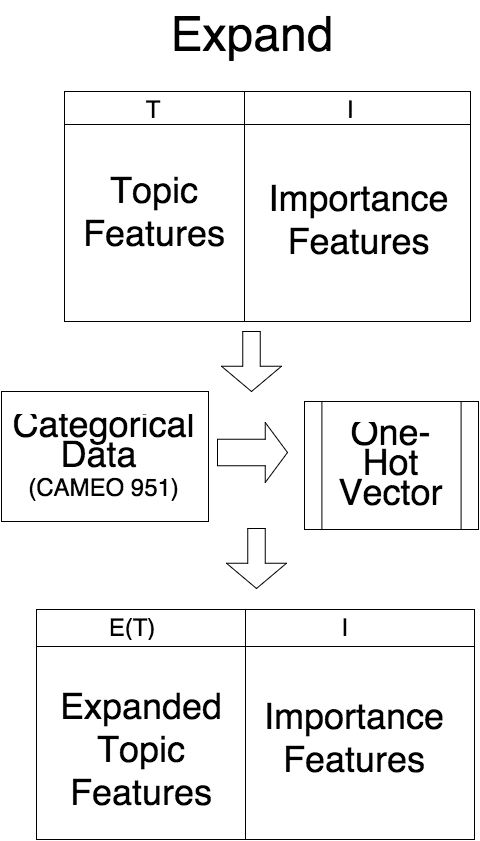
\includegraphics[scale=0.15]{images/expand_vertical.png}}
\caption{Expansion stage}
\end{center}
\vskip -0.2in
\label{fig:exapand}
\end{figure}

Expansion uses one-hot encoding on categorical features, such as the event CAMEO codes.

%TODO mention here that we do sample-mean and sample-std-dev-based scaling, once we actually do that

\begin{figure}[ht]
\vskip 0.2in
\begin{center}
\centerline{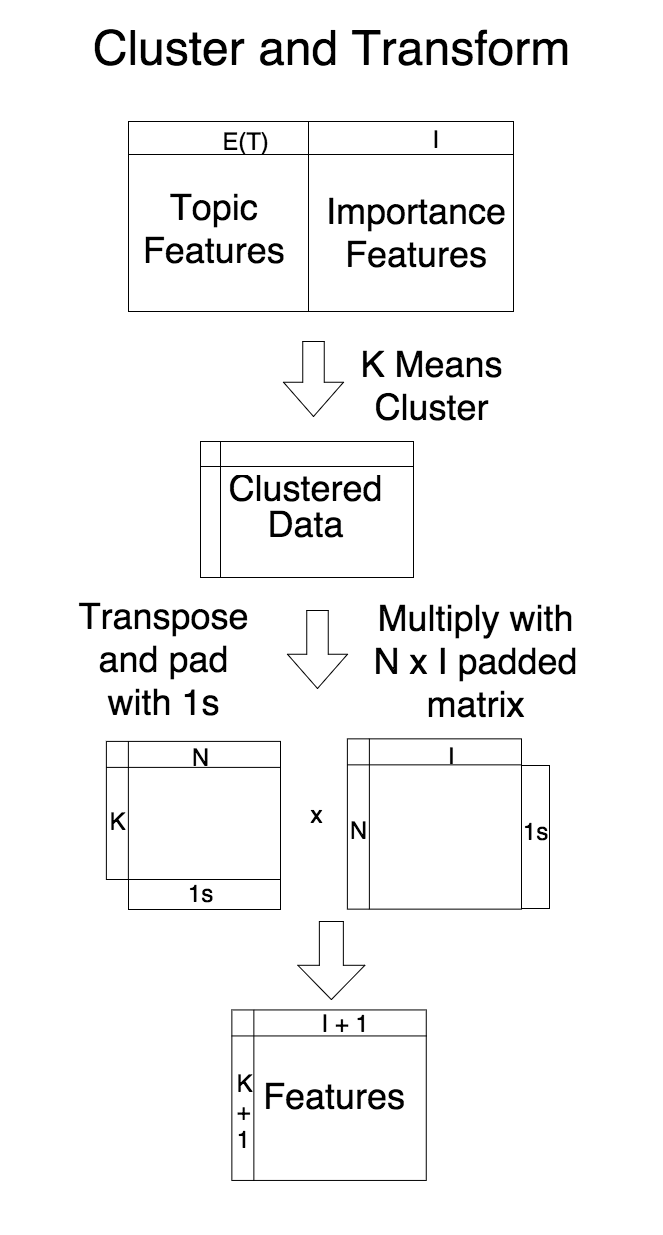
\includegraphics[scale=0.15]{images/cluster_and_transform_vertical.png}}
\caption{Summary stage}
\end{center}
\vskip -0.2in
\label{fig:summarization}
\end{figure}

The matrix multiply above conveniently extracts the sum of importance-weighted events belonging to certain topics. Note that this model is extensible to a mixture model, where each event's contribution to a topic's importance for that day is weighed by the probability of belonging to that topic's class. Furthermore, the aggregation creates a uniform description of every day, a flattened vector of dimension dependent on the cluster count.

These daily summaries were then enriched with historical pricing data before being fed into the linear model. The pricing data added was the 5, 10, and 30 day rolling average of the commodity price. %TODO hyperparam selection of rolling mean.
